\chapter{Collector - Bedienungsanleitung}
\label{appendix:collector}
\section{Startbildschirm}
Nach Start der Anwendung befindet man sich auf dem Startbildschirm:
\begin{figure}[H]
\centering
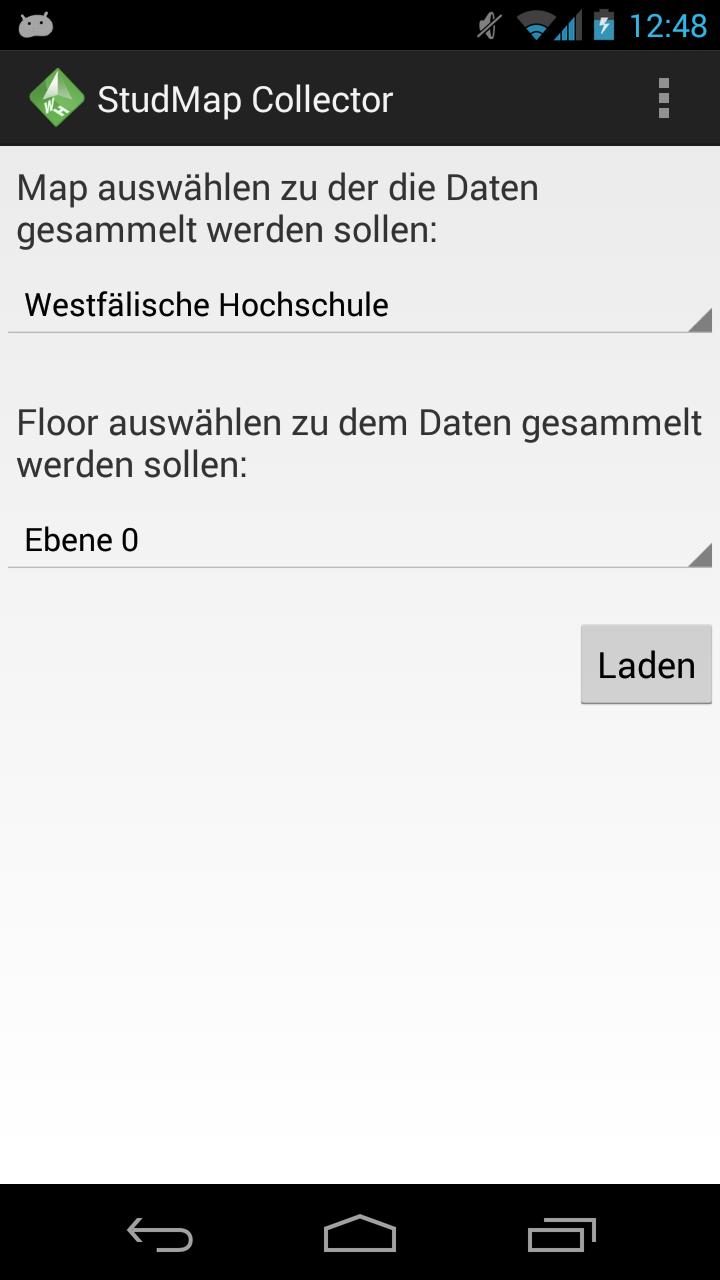
\includegraphics[width=0.5\linewidth]{../Bilder/Collector/StartScreen}
\label{fig:StartScreen}
\end{figure}
Hier k�nnen Karte und Stockwerk f�r die Datenerfassung ausgew�hlt werden. �ber den Button Laden wird die entsprechende Auswahl geladen.

\newpage

\section{Stockwerkansicht}
Hier sieht man das ausgew�hlte Stockwerk mit den zur Verf�gung stehenden Datenpunkten, die gr�n dargestellt sind.
\begin{figure}[H]
\centering
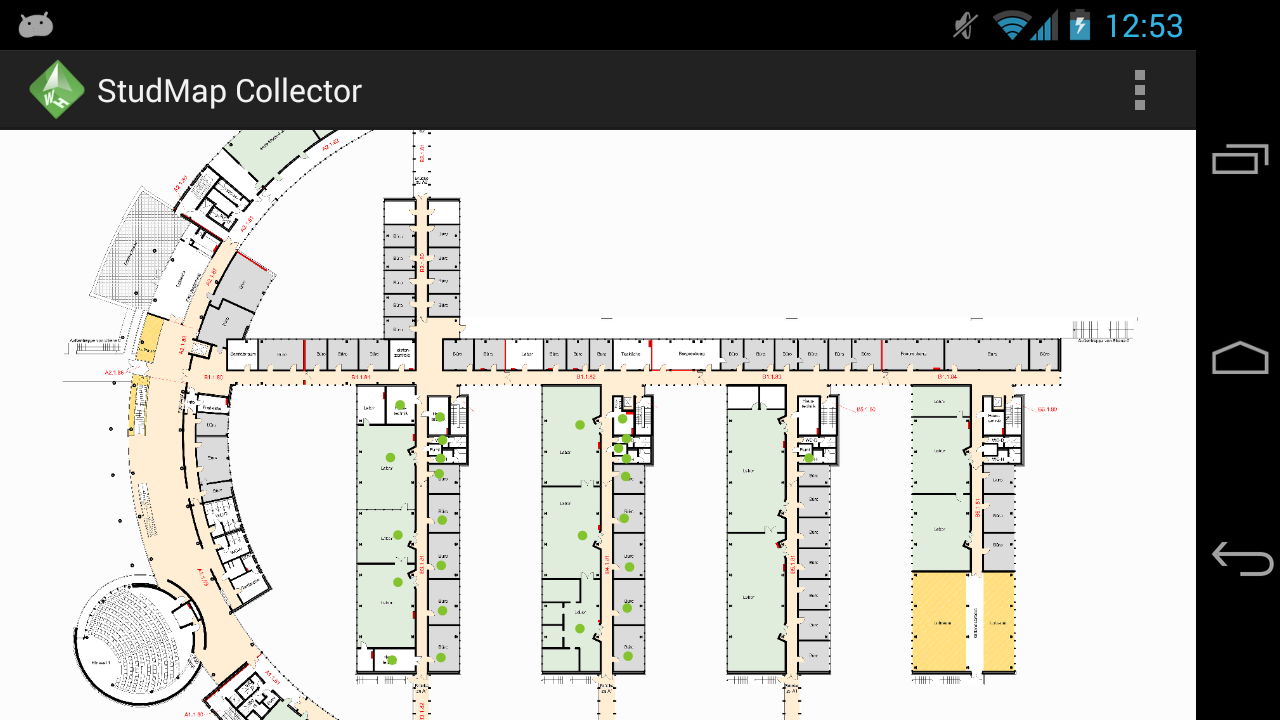
\includegraphics[width=0.8\linewidth]{../Bilder/Collector/FloorScreen}
\label{fig:FloorScreen}
\end{figure}

\subsection{Datenpunktauswahl}
Bei der Auswahl eines Datenpunktes erscheint folgender Dialog:
\begin{figure}[H]
\centering
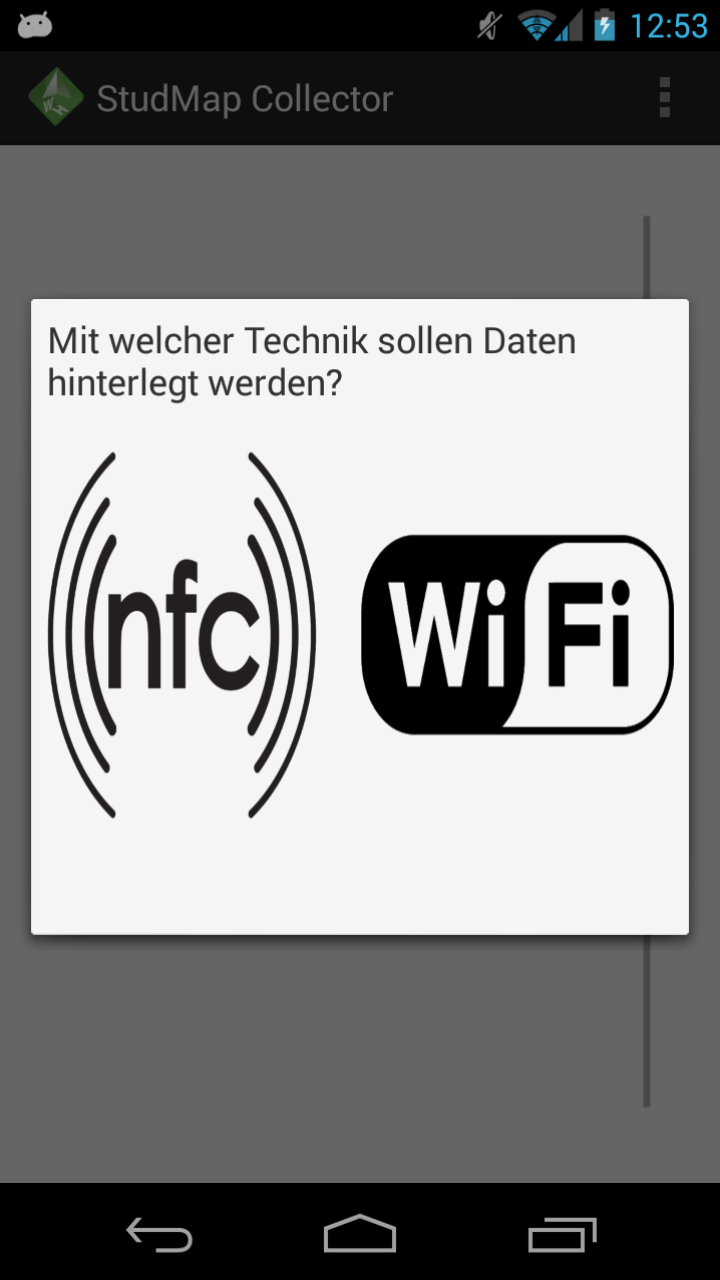
\includegraphics[width=0.35\linewidth]{../Bilder/Collector/StoreDataScreen}
\label{fig:StoreDataScreen}
\end{figure}
�ber diesen Dialog k�nnen f�r den ausgew�hlten Datenpunkt Positionsdaten hinterlegt werden. Dazu stehen die beiden Techniken NFC und Wifi zur Verf�gung.

\subsubsection{NFC-Tag Ansicht}
Solange das Ger�t keinen Kontakt zu einem NFC Tag hat, wird nur die ID des Datenpunkts ausgegeben.
\begin{figure}[H]
\centering
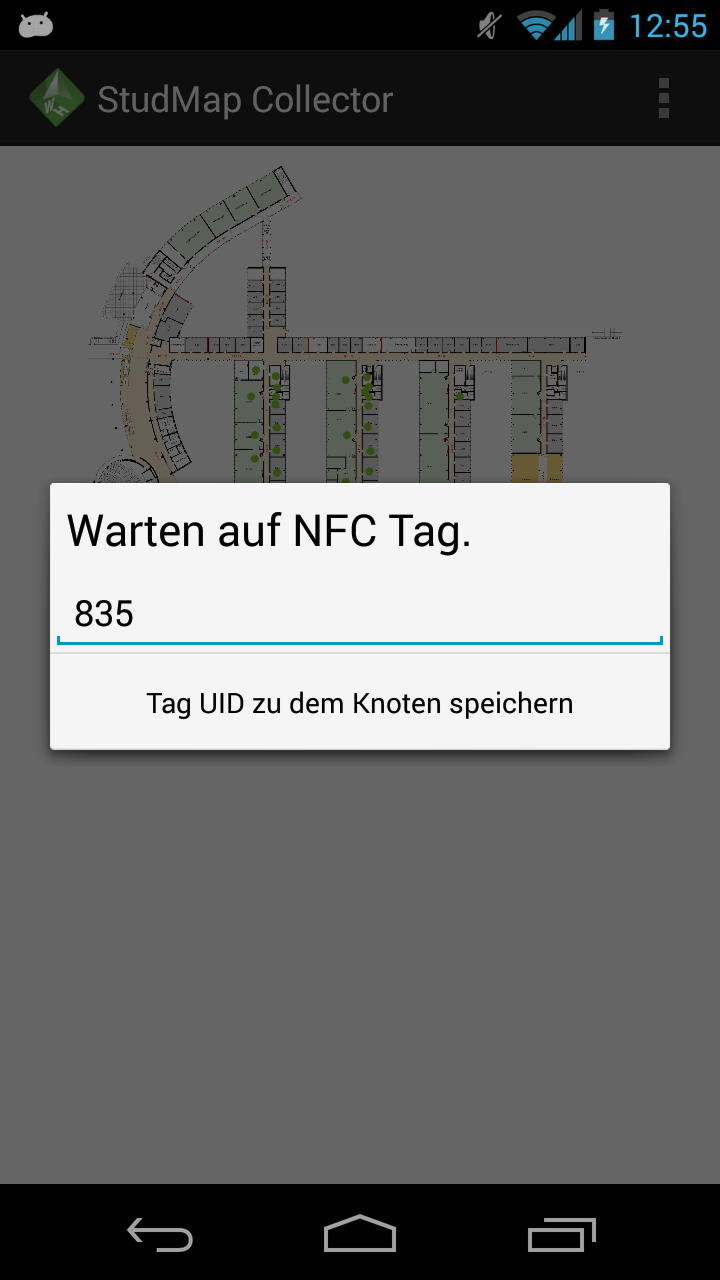
\includegraphics[width=0.35\linewidth]{../Bilder/Collector/NfcScreen}
\label{fig:NfcScreen}
\end{figure}

Sobald ein NFC Tag gefunden wurde, wird auch die ID des NFC-Tags im Dialog angezeigt und der Datenpunkt kann mit dem NFC-Tag verkn�pft werden.
\begin{figure}[H]
\centering
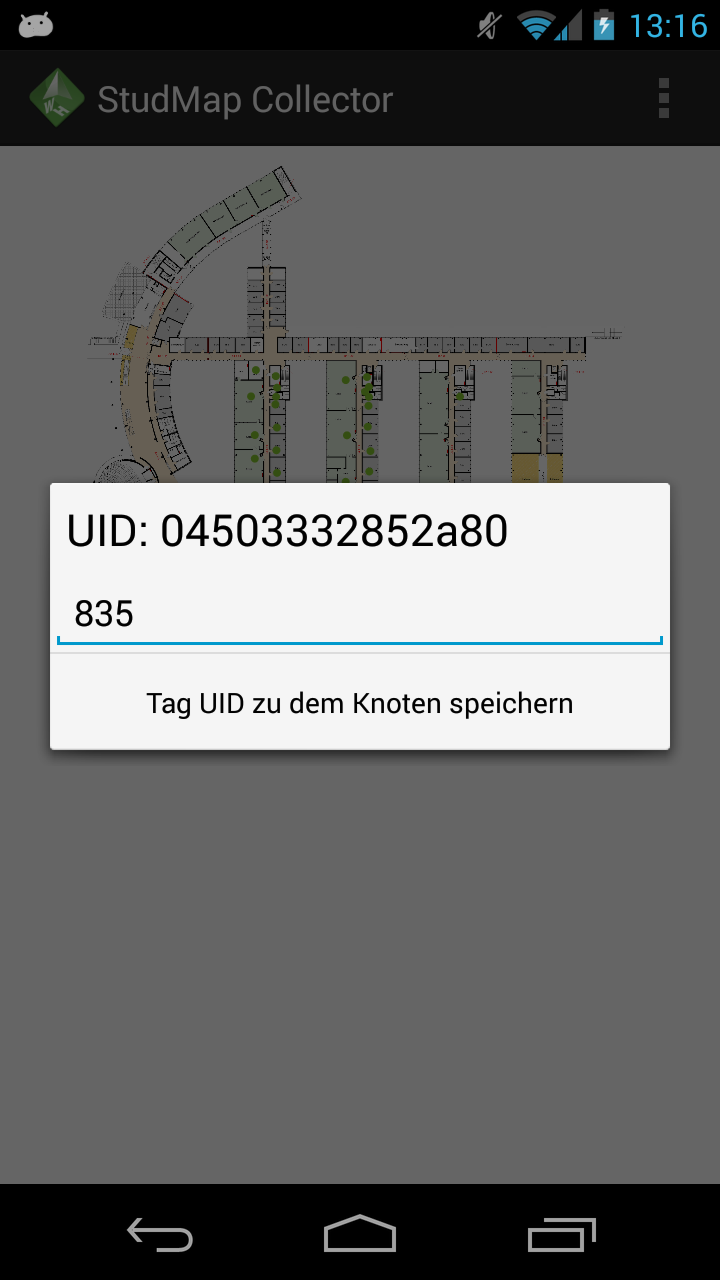
\includegraphics[width=0.35\linewidth]{../Bilder/Collector/NfcScreenRead}
\label{fig:NfcScreenRead}
\end{figure}

\newpage

\subsubsection{Wifi}
�ber diesen Dialog kann f�r den ausgew�hlten Datenpunkt ein WLAN-Fingerprint erstellt und gespeichert werden.
\begin{figure}[H]
\centering
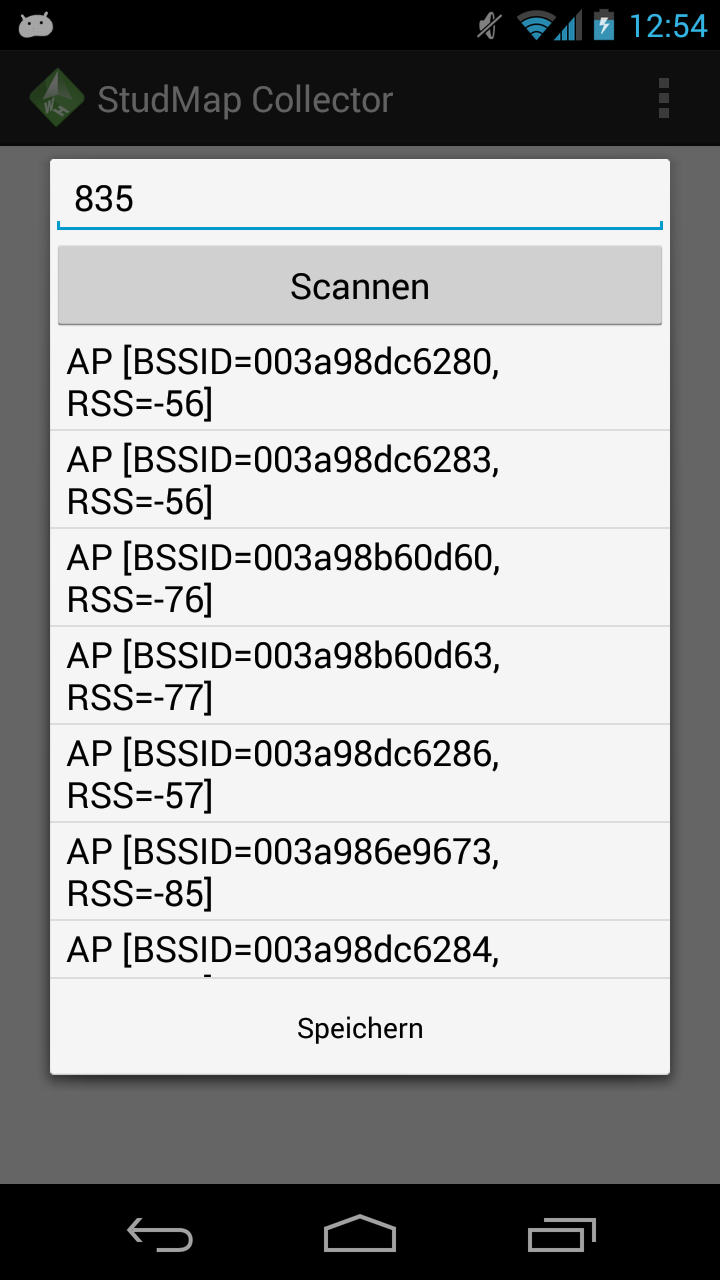
\includegraphics[width=0.5\linewidth]{../Bilder/Collector/WifiScannedScreen}
\label{fig:WifiScannedScreen}
\end{figure}
